\subsection{Thin layer entrainment}\label{sec:thin}
This experiment is performed as originally proposed by \citet{vanKeken1997} with two incompressible fluids in a rectangular domain with $L_x=2$ and $L_y=1$
and gravity acceleration $g_y=10^{10}Ra$. The Rayleigh number and the compositional Rayleigh number are fixed to $Ra=300000$ and $Rc=450000$, respectively.
Both fluids have constant viscosity, thermal conductivity, specific heat ($\eta=\rho=C_p=1$) and thermal expansion coefficient ($\alpha=10^{-10}$). Fluid 1
has a density $\rho_1=1$, while fluid 2 is denser ($\rho_2=\rho_1+1.5 \cdot 10^{-10}$) and is placed at the bottom of the domain, for $y \leq 0.025$.
Temperature are set to 0 on top and 1 on bottom of the domain. Velocity boundary conditions are set to free slip on all sides of the domain. The initial
temperature field is given by
\[T(x,y)=T_u(x,y)+T_l(x,y)+T_r(x,y)+T_s(x,y)-\frac{3}{2}\]
with
\begin{eqnarray}
T_u(x,y)&=&\frac{1}{2}erf\left(\frac{1-y}{2}\sqrt{\frac{u_0}{x}}\right)\nonumber \\
T_l(x,y)&=&1-\frac{1}{2}erf\left(\frac{y}{2}\sqrt{\frac{u_0}{L_x-x}}\right)\nonumber \\
T_r(x,y)&=&\frac{1}{2}+\frac{Q}{2\sqrt{\pi}}\sqrt{\frac{u_0}{y+1}} \exp\left(-\frac{x^2u_0}{4y+4}\right)\nonumber \\
T_s(x,y)&=&\frac{1}{2}-\frac{Q}{2\sqrt{\pi}}\sqrt{\frac{u_0}{2-y}} \exp\left(-\frac{(L_x-x)^2u_0}{8-4y}\right)\nonumber
\end{eqnarray}
and
\begin{eqnarray}
u_0&=&\frac{L_x^{7/3}}{(1+L_x^4)^{2/3}}\left(\frac{Ra}{2\sqrt{\pi}}\right)^{\frac{2}{3}}\nonumber \\
Q&=&2\sqrt{\frac{L_x}{\pi u_0}}\nonumber
\end{eqnarray}

The experiment is performed with two grid resolution ($125\times40$ and $200\times80$ elements), with 100 markers per element and CFL of 0.25. $v_{\textrm{rms}}$
(see Sec. \ref{sec:error}) calculated for both the simulations match well with results from \citet{vanKeken1997} and obtained with ASPECT
\citep{Kronbichler2012,Heister2017,Bangerth2020,Bangerth2020a} and ELEFANT \citep{Thieulot2014}, obtained with similar grid resolutions
(Fig. \ref{fig:thin}). In addition, a variety of simulations with different resolutions and aspect ratios are performed to verify that the sensitivity of the
initial velocity field. Results match well with results from \citet{vanKeken1997} (in the grey area) and \citet{Thieulot2014} (Fig. \ref{fig:thin_initial}). 
All data can be found at \url{https://github.com/aleregorda/Benchmarks/tree/main/Momentum%2BEnergy/Thin_layer}.

\begin{figure}
\centering
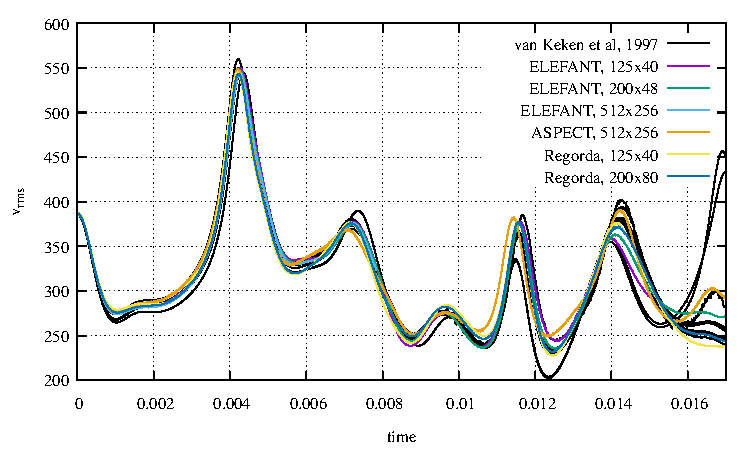
\includegraphics[width=400px]{./Figures/vrms_thin.pdf}
\caption{$v_{\textrm{rms}}$ for the thin layer experiment as function of time for different grid resolution. Results are compared with results obtained by
\citet{vanKeken1997} (black lines) and with ASPECT and ELEFANT.}
\label{fig:thin}
\end{figure}

\begin{figure}
\centering
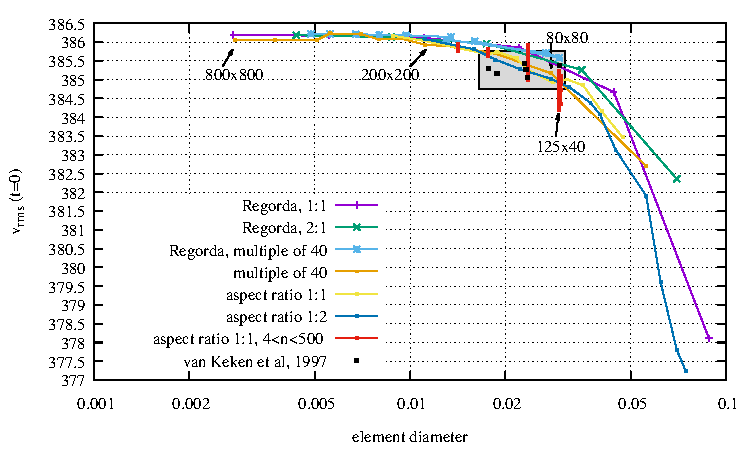
\includegraphics[width=400px]{./Figures/vrmszero.pdf}
\caption{$v_{\textrm{rms}}$ at $t=0$ for the thin layer experiment as function of the element size for different aspect ratios of the elements. Results are compared
with results obtained by \citet{vanKeken1997} (black dots in the grey area) and with ASPECT and ELEFANT.}
\label{fig:thin_initial}
\end{figure}